\chapter{De architectuur van het proof of concept}\label{chap: currentState}
Dit hoofdstuk onderzoekt naar de geschikte software architectuur voor het proof of concept en beantwoord hierdoor de vraag \researchQuestionTwo (\textbf{SRQ2} uit paragraaf \ref{chap:researchQuestions}). Om hier antwoord op te geven word de vraag in de volgende subvragen verder opgesplitst in: 
\begin{enumerate}
	\item Wie zijn stakeholders van het proof of concept en wat zijn hun algemene belang?
	\item Wat zijn de requirements?
	\item Welke technologieën beste geschikt voor de proof of concept use case?
\end{enumerate}

De resultaten op deze vragen die worden gepresenteerd in dit hoofdstuk defineren gelijk het design van het proof of concept (PoC). Technologie keuzes worden in paragraaf \ref{decisionForcesView} behandeld. De C4 \footnote{https://c4model.com/} software architectuur modeleer methodiek die is ontwikkeld door Simon Brown wordt gebruikt in dit proces.

\newpage

\section{Functionele en non-functionele requirements}\label{requirements}
De scope van de implementatie beschreven beperkt zich tot de volgende gebruikers:
verzekeraar, verzekerde, makelaar en administrator. Om zo compleet mogelijk alle functionele requirements te noteren zijn de user stories in de onderstaande tabel \ref{fig:userstories} vanuit de verschillende gebruikers perspectief geschreven. Hiermee beantwoorden we gelijk de vraag wie de stakeholders zijn in het systeem en wat hun belangen zijn.\par

Er is tijdens het opstellen van deze requirements gekozen om alleen het essentiële op te schrijven en deze zoveel mogelijk de versimpelen. Te weten dat, het quality attributes zoals het gebruiksgemak en security eisen van de PoC op een rendabel niveau moeten zijn.

\begin{figure}[h!]
    \begin{center}
        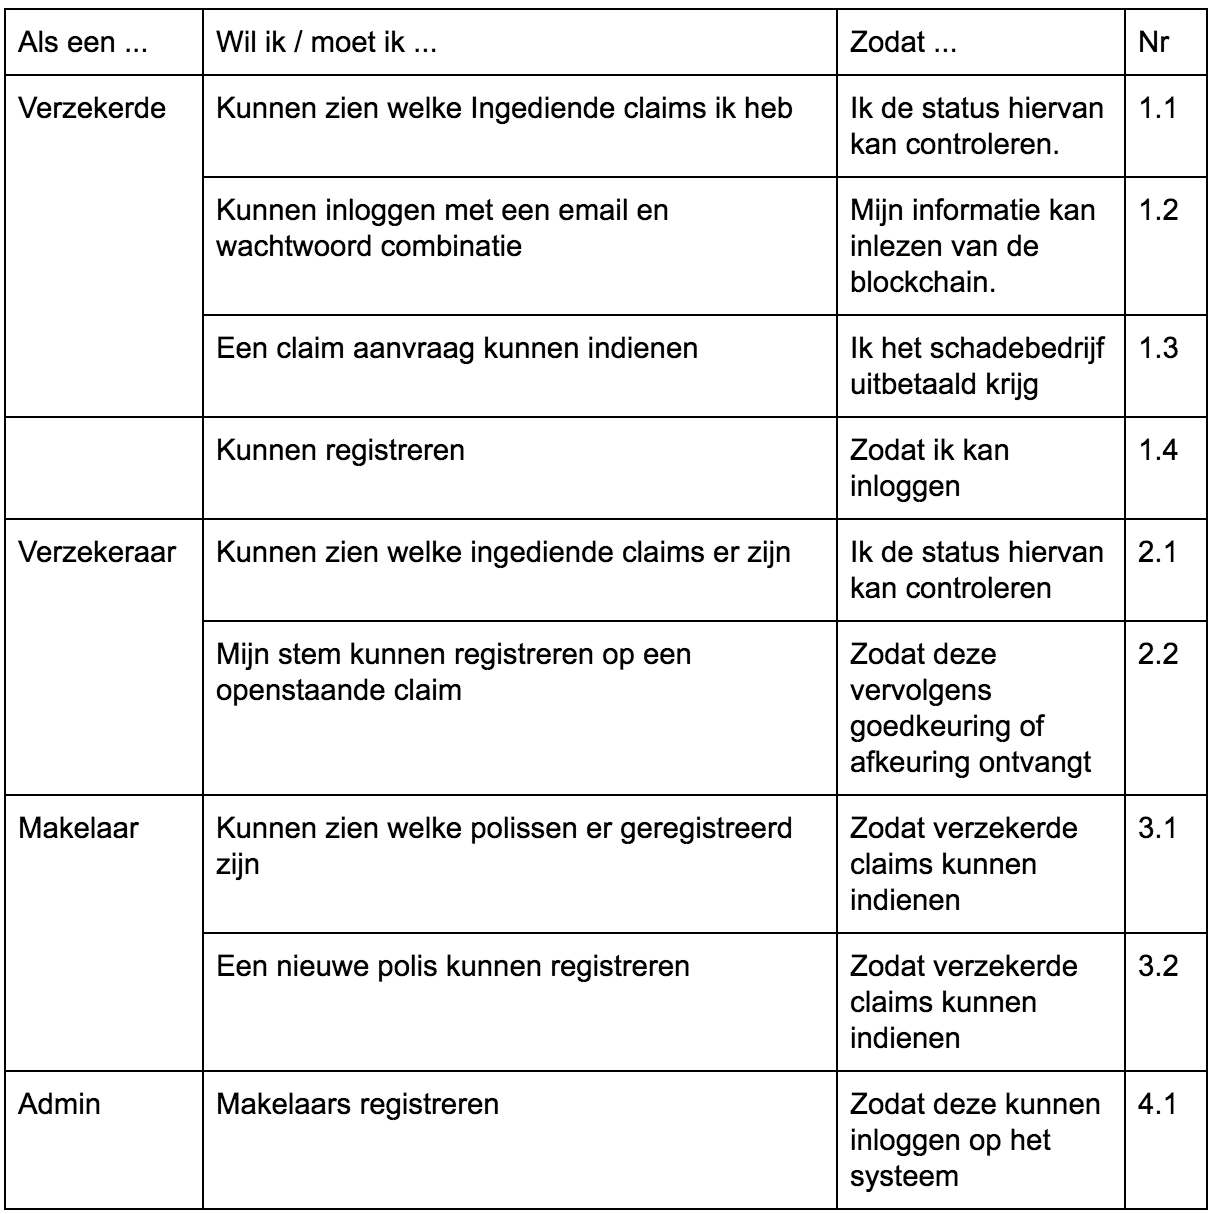
\includegraphics[scale=0.7]{images/userstories}
        \caption{User stories die de functionele requirements defineren.}
        \label{fig:userstories}
    \end{center}
\end{figure}
\newpage

\subsection{Overige Requirements}
In de onderstaande opsomming staan overige requirements die ook aan het PoC worden gesteld.
\begin{itemize}
  \item \textbf{R1.} Het systeem geeft gebruikers toegang op basis van hun email en wachtwoord.
  \item \textbf{R2.} Het systeem controleert bij een claim aanvraag van of het polis nummer valide is
  \item \textbf{R3.} Het systeem moet automatisch goedkeuring geven voor een claim als het claimbedrag onder 1000 euro zit en het type diefstal is.
  \item \textbf{R4.} Met gebruik van smart contracts en de blockchain wordt de data integriteit gewaarborgd.
  \item \textbf{R5.} Een verzekeraar kan bij het aanmaken van een nieuwe polis aangeven wat de verdeling is tussen de verzekeringsmaatschappijen.
  \item \textbf{R6.} Het systeem ondersteund Ruitschade, Brandschade, Stormscade en diefstal als types voor een claim aanvraag.
  \item \textbf{R7.} Een claim is via de blockchain te verifiëren.
  \item \textbf{R8.} Nadat alle verzekeraars een claim aanvraag hebben goed gekeurd word de claim automatisch op status goedgekeurd gezet.
  \item \textbf{R9.} Een claim kan alleen de open, in behandeling, goedgekeurd, afgewezen en automatisch goedgekeurd statussen hebben.
  \item \textbf{R10.} Het systeem geeft per claim aan op hoeveel goedkeuringen het wacht en nog nodig heeft.
  \item \textbf{R11.} Wanneer een verzekeraar een claim weigert word de claim automatisch op status afgewezen gezet.
  \item \textbf{R12.} A transcation should not take more than 5 minutes.
  \item \textbf{R13.} Het systeem slaat de claims gedecentraliseerd op. Er zijn dus geen centrale punten van controle.
  \item \textbf{R14.} Het systeem schaalt met de groei van gebruikers mee zonder dat het systeem langzamer word.
  \item \textbf{R15.} Gebruikers hebben interactie met het systeem via een web interface.
\end{itemize}
\newpage

\subsection{Context - Actors en hun High-level Use Cases}
In het onderstaande diagram zijn de actors te zien. Het laat zien hoe deze gebruikers/systemen met het systeem communiceren.
\begin{figure}[h!]
    \begin{center}
        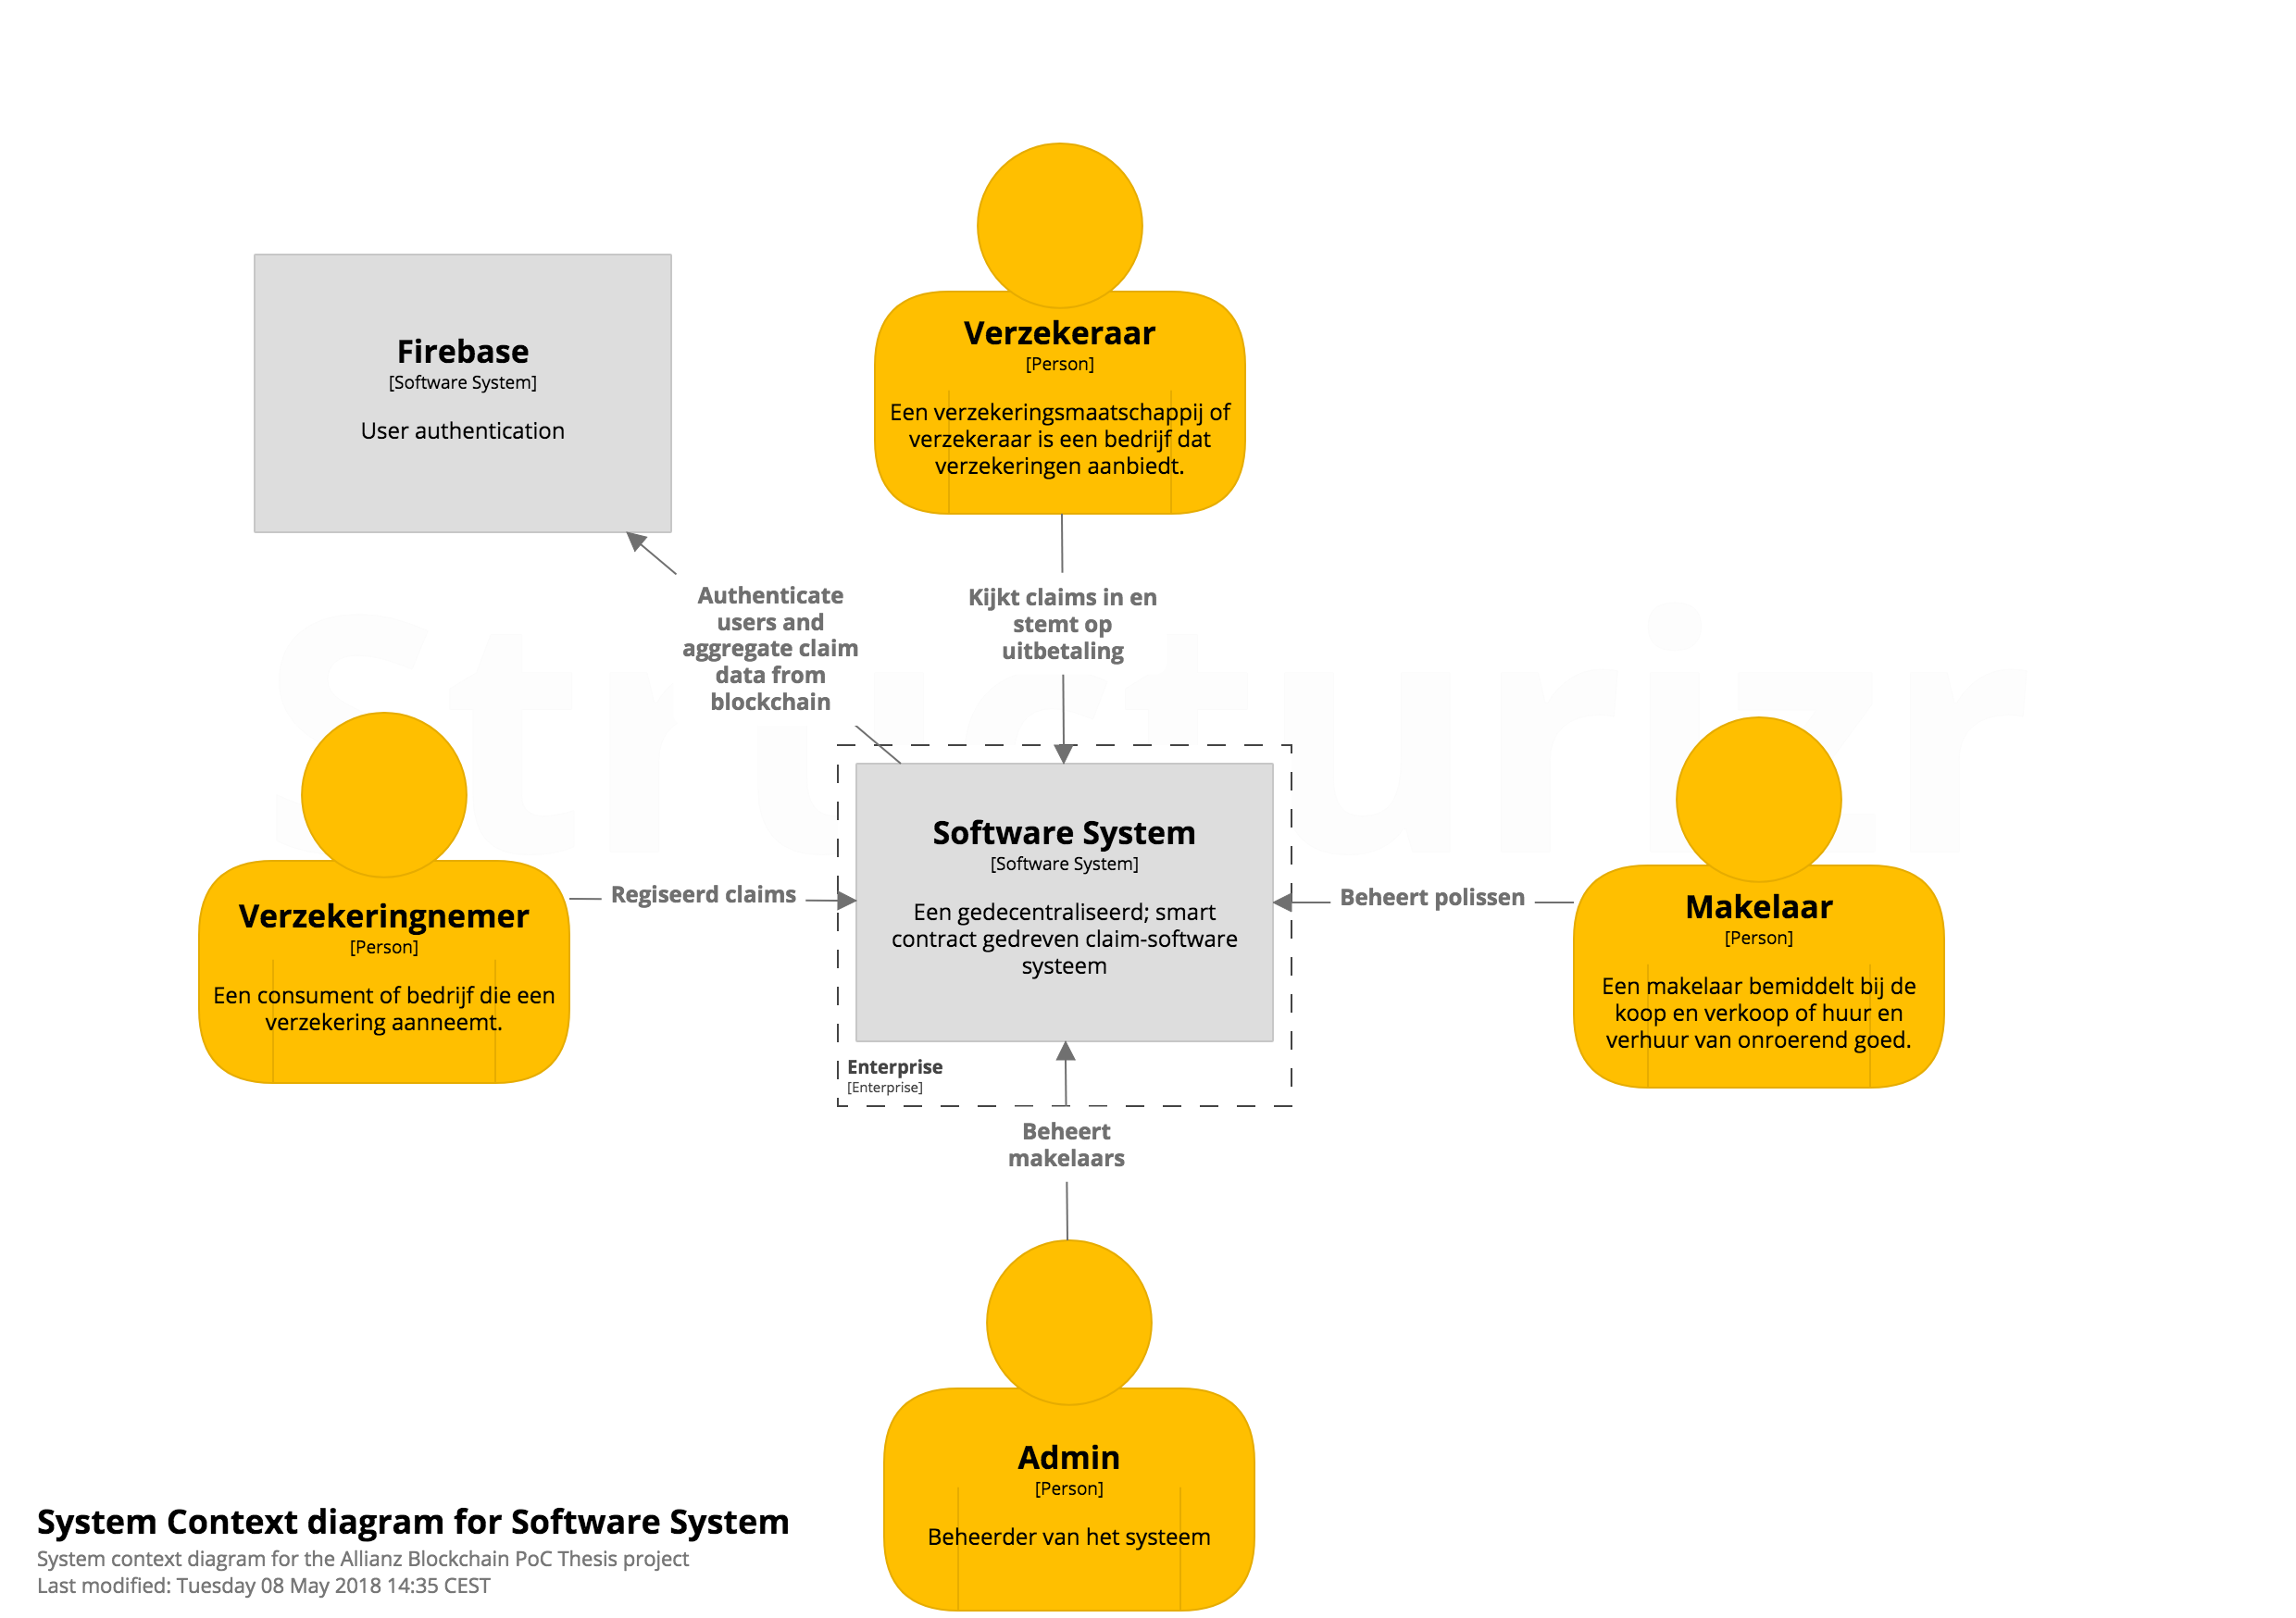
\includegraphics[width=\paperwidth-200]{images/context}
        \caption{C4 - Context.}
        \label{fig:c4Context}
    \end{center}
\end{figure}

In de onderstaande tabel worden de actors beschreven.
\begin{figure}[h!]
    \begin{center}
        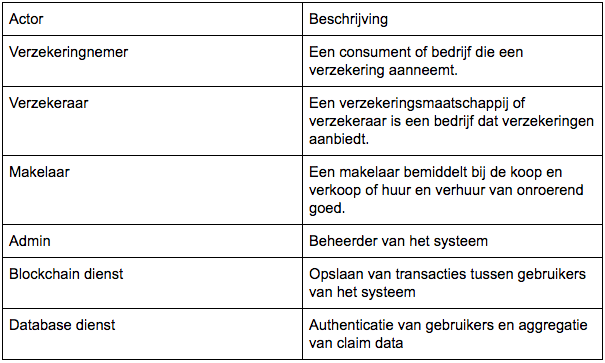
\includegraphics[width=\paperwidth-250]{images/actors}
        \caption{Actors in het systeem}
        \label{fig:actors}
    \end{center}
\end{figure}

\newpage

\section{Decision forces view}\label{decisionForcesView}
Een decision force is een term die ik tijdens het Advanced Software Development semester heb geleerd. Een force is een beslissingsfactor van een architectureel probleem dat zich in het systeem of zijn omgeving. In de context van dit project is het de blockchain technologie keuze waarop het proof of concept op wordt gebouwd. Deze decision forces kunnen vanuit viewpoints komen, zoals: operationeel, ontwikkeling, zakelijk, organisatorisch, politiek, economisch, juridisch, regelgevend, ecologisch, sociaal \cite{architectureForces}. Uiteindelijk word een decision force gekoppeld aan een system quality attribute die de verschillende concerns aantoont. Hiermee worden uiteindelijk de verschillende technologieën vergeleken. De volgende decision forces zijn in samenwerking met Allianz, de stakeholder van het proof of concept samengesteld naast de requirements die in paragraaf \ref{requirements} zijn behandeld.

\begin{itemize}
  \item \textbf{F1.} 
  \item \textbf{F2.} 
  \item \textbf{F3.} 
  \item \textbf{F4.} 
  \item \textbf{F5.} 
  \item \textbf{F6.} 
  \item \textbf{F7.} 
  \item \textbf{F8.} 
\end{itemize}

Zie de bijlagen \cite{appendix:decisionForcesView} waar de decision forces view te zien is.

\newpage

\section{Container diagram}

\begin{figure}[h!]
    \begin{center}
        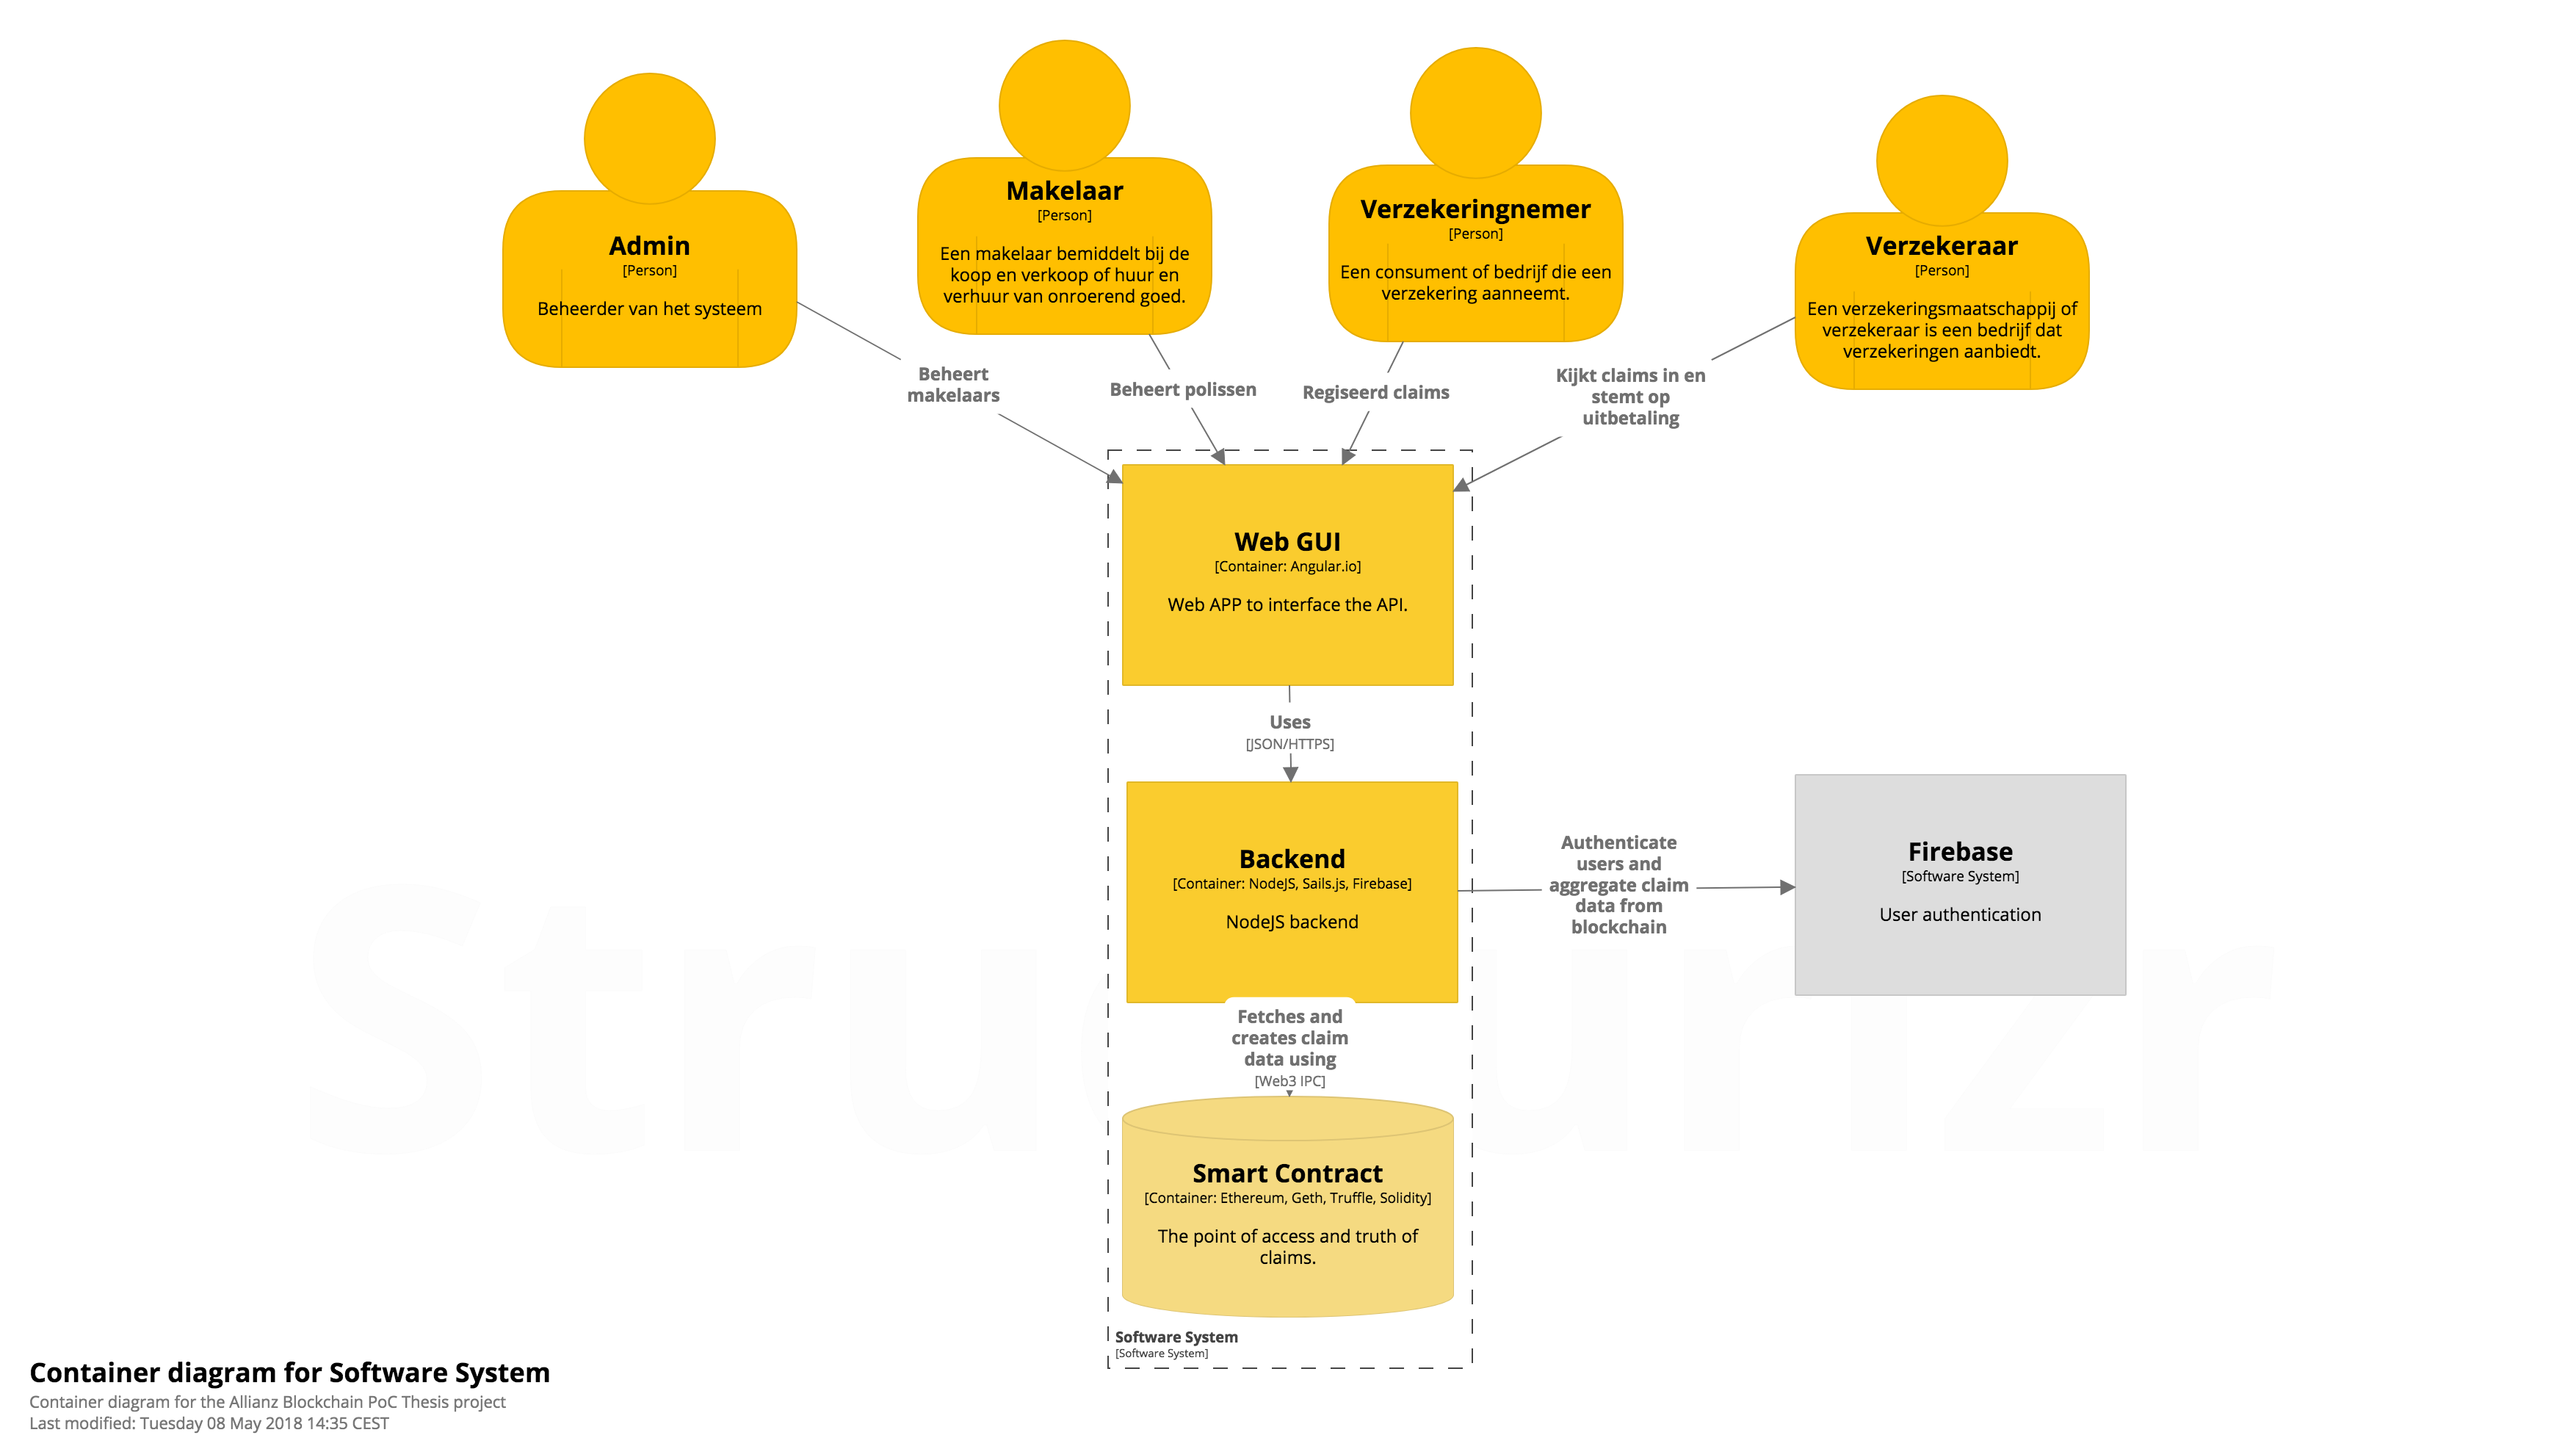
\includegraphics[width=\paperwidth-100]{images/containers}
        \caption{C4 - Containers.}
        \label{fig:c4Containers}
    \end{center}
\end{figure}
